\chapter{評価}
\label{evaluation}
本章では,提案システムの評価に大きく二つ述べる。一つは他の活性化関数との比較。もう一つは、

\section{評価内容}


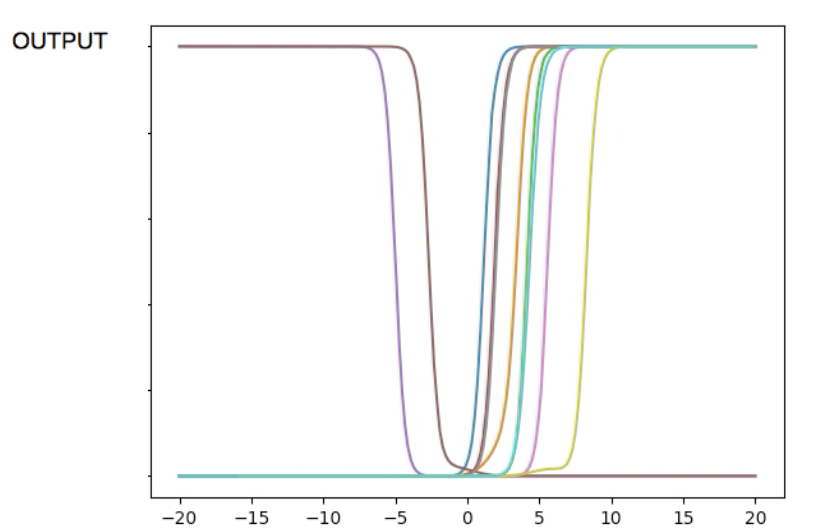
\includegraphics[width=5cm]{asset/output.png}
色々実験結果の活性化関数を乗っけていく

ここまで 10 つの実験を行い, 潜在変数空間の構築精度, データ生成能力, 潜在変数空間と
観測データ空間における分散の有用性の観点から先行研究との比較を行った. 実験結果を
踏まえ, 第 6 章で考察を行う.




%%% Local Variables:
%%% mode: japanese-latex
%%% TeX-master: "./thesis"
%%% End:
